\pdfoutput=1
\documentclass[11pt]{article}
\usepackage[margin=1in]{geometry}
\usepackage{booktabs}
\usepackage{amsmath,amssymb}
\usepackage{tabularx}
\usepackage{microtype}
\usepackage{xspace}
\usepackage{tikz}
\usetikzlibrary{positioning,arrows.meta,calc}
\usepackage{pgfplots}
\pgfplotsset{compat=1.18}
\usepgfplotslibrary{groupplots}
\usetikzlibrary{patterns,shapes.geometric}
% Figure palette: one hue per framework (validated categorical pair; CVD dE 24.7,
% normal-vision dE 33.6, >=3:1 on white), neutral inks for all text and chrome.
\definecolor{sglang}{HTML}{2A78D6}
\definecolor{vllm}{HTML}{EB6834}
\definecolor{inksec}{HTML}{52514E}
\definecolor{inkmuted}{HTML}{898781}
\definecolor{gridc}{HTML}{E1E0D9}
\definecolor{axisc}{HTML}{C3C2B7}
\definecolor{panel}{HTML}{F5F4F0}
\usepackage[numbers,sort&compress]{natbib}
\usepackage[hidelinks]{hyperref}
\hypersetup{pdftitle={No Permanent Champion: A Deployment Study of SGLang and vLLM across Dense, Ultra-Sparse MoE, and KDA-Hybrid Architectures on H200 GPUs}, pdfauthor={Chao-Chun Chuang, Po-Hsiang Lin, Liang-Hsun Huang}}
\usepackage{url}

\newcommand{\tps}{tok/s\xspace}
\newcommand{\figsub}[1]{{\footnotesize\color{inksec}#1}}

\title{\textbf{No Permanent Champion: A Deployment Study of SGLang and vLLM across Dense, Ultra-Sparse MoE, and KDA-Hybrid Architectures on H200 GPUs}}

\author{
Chao-Chun Chuang$^{1,\ast}$, Po-Hsiang Lin$^{2}$, and Liang-Hsun Huang$^{3}$\\[4pt]
\small $^{1}$National Center for High-performance Computing (NCHC),\\
\small National Institutes of Applied Research (NIAR), Taiwan\\
\small $^{2}$Kaohsiung Veterans General Hospital, Kaohsiung, Taiwan\\
\small $^{3}$Twinkle AI, Taiwan\\[2pt]
\small $\ast$ Corresponding author: \texttt{c00cjz00@nchc.org.tw}
}
\date{September 2026}

\begin{document}
\maketitle

\begin{abstract}
\noindent We operate a multi-model API service on an HPC cluster---a LiteLLM gateway fronting Slurm-managed SGLang and vLLM engines on NVIDIA H200 GPUs---and each new model it onboards raises the same question: which serving framework will run this checkpoint faster? We encoded the comparison as versioned procedures (``skills'') that an LLM-based agent executes under human approval: both frameworks' engines are scaffolded from official per-model documentation, deployed side by side under traffic-isolated aliases, and driven with the same 500--1,000-request burst in five repetitions under an interleaved, warmed-up protocol (with one documented rerun exception). Across three 2026 models---a 27B dense hybrid, a 180B-total/6B-active ultra-sparse MoE, and a 288-expert Kimi Delta Attention (KDA) hybrid MoE---the leader depended on the architecture: SGLang led the dense model by 9.6\% on average and in every paired repetition, while vLLM led the MoE by 2.40$\times$ and the KDA hybrid by 28\% (30\% across four independent engine-instance pairs). In each framework's deployable configuration, speculative decoding with the checkpoints' integrated draft heads lowered throughput in five of six framework--model pairs, by up to 49\%. For SGLang on the dense model the loss came from memory rather than computation: with EAGLE's footprint, 80 was the highest concurrency cap that started in our sweep, whereas at equal concurrency EAGLE raised throughput by 15\%. An earlier single run without warm-up had reversed the KDA ranking, understating vLLM by 39\%; warm-up and repetition recovered it. An agent-assisted layered diagnosis also raised mixed 1,500-user success from 67.9\% to 100\% by correcting file-descriptor limits. Framework choice and speculative decoding should therefore be measured per model, with repetition, rather than inherited as defaults; the procedure and the raw measurements behind the comparisons are released.
\end{abstract}

\section{Introduction}

The throughput and latency of a deployed large language model (LLM) depend not only on the model and the accelerator, but on the serving framework that schedules batches, manages KV-cache memory, and executes attention and mixture-of-experts (MoE) kernels. Among open-source serving frameworks, a study of open-source software systems found vLLM to be the most visible in popularity and adoption, with SGLang among its principal alternatives~\cite{majidi2026wild}. vLLM was introduced with PagedAttention for efficient KV-cache memory management~\cite{kwon2023vllm}, and SGLang with a RadixAttention prefix cache and a structured-generation runtime~\cite{zheng2024sglang}. Both systems evolve quickly, add support for new model architectures as they appear, and make different implementation trade-offs for the same architecture. Practitioners therefore face a recurring question that vendor documentation does not answer: \emph{for this specific model, on this hardware, which framework will serve it faster?}

This question is not academic for us. We operate a multi-model API service for the users of an HPC cluster: a LiteLLM gateway fronting Slurm-managed inference engines---SGLang and vLLM containers among them---on NVIDIA H200 GPUs, with per-engine lifecycle management, versioned container images, and declarative routing that lets a candidate engine receive production-shaped traffic under isolated aliases before it claims any production name. Every time the center onboards a new open-weight model, the platform forces a concrete framework decision, and the wrong one is expensive: as this paper shows, the cost of choosing wrongly reaches 2.4$\times$ in throughput---larger than any tuning lever we measured, including correcting an outright misconfiguration (+48\% on the dense engine's earlier settings). Manual evaluation is slow and error-prone (framework-specific flags, memory budgets, and validation steps differ), so we delegated it to an agent: the evaluation procedure---engine scaffolding from each framework's official per-model documentation, dual-framework deployment, paired benchmarking, verdict recording, and production traffic switching---was encoded as declarative, versioned procedures (which we call \emph{skills}) and executed by an LLM-based coding agent under human approval.

Published comparisons between serving systems do exist: an empirical evaluation of vLLM against HuggingFace TGI on LLaMA-2 models is a recent example~\cite{kolluru2025tgi}, surveys consolidate the serving-systems literature~\cite{li2024survey}, and a study of open-source deployments documents which frameworks practitioners actually adopt~\cite{majidi2026wild}. Same-checkpoint comparisons of multiple backends have quantified accuracy fidelity~\cite{pape2026silent}, and SiliconBench evaluates nine Apple Silicon serving engines on unified-memory desktops, using CUDA vLLM and SGLang as references~\cite{zhang2026siliconbench}; neither addresses throughput at hundreds to a thousand concurrent requests on HPC GPUs, and none evaluates ultra-sparse MoE or KDA hybrids. Separately, the fragility of speculative decoding under batched serving is not merely a vendor warning: goodput analyses and adaptive speculation control have formalized when drafting helps and when it hurts~\cite{liu2024turbospec,li2025adaserve}. What remains unmeasured is how these framework and speculation choices behave on the newest architectures---with checkpoint-integrated multi-token prediction (MTP) heads rather than external draft models---under high-concurrency burst load.

The present paper reports what this agent-assisted workflow found, together with the workflow itself. We make five contributions:

\begin{enumerate}
\item \textbf{An agent-assisted evaluation workflow} (Sections~3--4): a paired A/B procedure---both frameworks serving the \emph{same local checkpoint} on the same GPU type under the \emph{same client workload}, with engine parameters taken from official documentation, five repetitions under an interleaved, warmed-up protocol (one documented exception; Section~\ref{sec:method}), and every run's statistics recorded---encoded as versioned skills that an LLM-based agent executes under human approval, from scaffolding the candidate engine to switching production traffic.
\item \textbf{Three per-model results} (Section~5): SGLang 0.5.20 led by 9.6\% on a dense 27B hybrid; vLLM 0.29.1rc1 led by 2.40$\times$ on a 180B/6B-active ultra-sparse MoE; and a dedicated vLLM 0.28.1rc1 build led by 28\% on a 306 GB FP8 KDA model---so the leading framework is model-specific, and the gap can outweigh every other tuning lever we measured.
\item \textbf{Speculative decoding under load} (Sections~\ref{sec:dense}--\ref{sec:synthesis}): in each framework's deployable configuration, the checkpoints' integrated draft heads lowered throughput in five of six framework--model pairs (by 7--49\%). A cap-48 control and a feasibility sweep show that for SGLang on the dense model the loss is a memory effect: EAGLE raises throughput by 15\% at equal concurrency, but the highest tested feasible cap is 80, where it still trails the plain configuration by 34\%.
\item \textbf{A measurement-protocol finding} (Sections~\ref{sec:kda} and~6): a single run without warm-up reversed the KDA ranking, understating vLLM by 39\%; with warm-up, all four independent engine-instance pairs favored vLLM, with cross-instance CVs of 1--2\%.
\item \textbf{A production platform description and reliability analysis} (Sections~3 and~\ref{sec:reliability}): a LiteLLM-based multi-engine gateway with Slurm-managed engine lifecycle, declarative production/staging traffic switching, and versioned container images, together with a layered diagnosis---also agent-assisted, from an encoded symptom-to-cause procedure---that traced mixed-load failures (67.9\% $\rightarrow$ 91.8\% $\rightarrow$ 100\%) to file-descriptor limits in the client shell and per-connection sshd, not to GPU engines or the gateway.
\end{enumerate}

All experiments were run in September 2026 on the platform described in Section~3; raw per-run and per-request data are released in the artifact repository (see Data and Artifact Availability).

\section{Related Work}

\textbf{Serving systems.} Iteration-level scheduling and continuous batching were introduced by Orca~\cite{yu2022orca} and adopted by vLLM, whose PagedAttention brought operating-system-style page management to KV-cache memory~\cite{kwon2023vllm}. SGLang contributed RadixAttention for automatic prefix reuse and an efficient runtime for structured generation programs~\cite{zheng2024sglang}. Chunked prefill, proposed in SARATHI, mitigates the interference of long prefills with decodes~\cite{agrawal2023sarathi}, and DistServe shows that disaggregating prefill from decoding improves goodput under latency constraints~\cite{zhong2024distserve}. Kernel libraries such as FlashInfer supply portable attention and decoding kernels that both frameworks integrate~\cite{ye2025flashinfer}. Our work does not propose a new serving mechanism; it measures two mature frameworks on a production platform and finds that their relative standing differs across the three models tested.

\textbf{Model architectures under test.} The three models we evaluate span the current design space of efficient open-weight LLMs. Qwen3.8-27B continues the dense hybrid line of Qwen3~\cite{yang2025qwen3}, combining gated delta net (GDN) linear attention with full attention. Qwen3.8-Flash-Next is an ultra-sparse MoE (180B total, 6B active parameters, 512 experts) with a large N-gram embedding table, in the lineage of DeepSeek-V2/V3's economical MoE and multi-head latent attention (MLA) designs~\cite{deepseek2024v3,deepseek2024v2}. GLM-5.3-Flash continues the GLM agentic line~\cite{glm2026glm5} as a native-FP8, 288-expert MoE (8 experts active per token, one shared expert, first three layers dense) whose 45-layer attention stack interleaves, three-to-one, 34 Kimi Delta Attention (KDA) linear-attention layers---the architecture introduced by Kimi Linear~\cite{kimi2025linear}---with 11 DeepSeek Sparse Attention (DSA) layers, plus a 1M-token context window; its closest published relatives include Kimi K2's large sparse-MoE design~\cite{kimi2025k2}, and serving-side research on KDA-style hybrids is already emerging---recurrent-state compression (DASC)~\cite{yu2026dasc}, decay-aware mixed-precision state quantization (DAMP)~\cite{zhang2026damp}, and switchable per-layer mixer placements, including KDA, served from one supernet checkpoint (Super Apriel)~\cite{slam2026superapriel}. The architectural diversity of this trio is a plausible reason framework rankings might not transfer across models---a hypothesis our results support but cannot isolate, given one model per architecture.

\textbf{Speculative decoding.} Speculative sampling accelerates autoregressive decoding by drafting multiple tokens with a cheap proposal mechanism and verifying them in parallel with the target model~\cite{leviathan2023spec}. Proposal mechanisms include additional decoding heads (Medusa~\cite{cai2024medusa}), feature-level draft models with uncertainty handling (EAGLE~\cite{li2024eagle}), and the checkpoint-integrated MTP heads of DeepSeek-V3~\cite{deepseek2024v3} and its successors, which both frameworks in this study expose as NEXTN/MTP options. The published literature evaluates speculative decoding primarily as a \emph{latency} optimization at low request concurrency~\cite{leviathan2023spec,li2024eagle,cai2024medusa}, but its behavior under batched serving has been studied: goodput analyses observe that speculation can degrade serving performance when applied without regard to load, and adaptive systems such as TurboSpec close the loop by enabling drafting only when it pays~\cite{liu2024turbospec}; AdaServe customizes speculation to per-request SLOs~\cite{li2025adaserve}. Our contribution is narrower and complementary: a repeated measurement of \emph{checkpoint-integrated} MTP/NEXTN heads across two frameworks and three architectures under high-concurrency burst load, with controls that distinguish the throughput lost to a reduced concurrency cap from the net effect of speculation at a fixed cap.

\textbf{Empirical comparisons of serving frameworks.} A comparative performance study of vLLM and HuggingFace TGI on LLaMA-2 models (7B--70B) found framework-dependent trade-offs in throughput, latency, and memory~\cite{kolluru2025tgi}; a survey consolidates the broader serving-systems literature~\cite{li2024survey}; and a large-scale analysis of open-source systems documents which serving frameworks and methods are adopted in practice~\cite{majidi2026wild}. The Silent Hyperparameter holds weights and decoding fixed across five backends but measures accuracy reproducibility rather than throughput~\cite{pape2026silent}; SiliconBench evaluates nine Apple Silicon serving engines on unified-memory desktop hardware, using CUDA vLLM and SGLang as references, with fidelity as a first-class metric~\cite{zhang2026siliconbench}; and AutoTuneBench has agent systems auto-tune both engines under a strict measurement protocol (paired seeds, cross-run CV at most 5\%)~\cite{chen2026autotunebench}. Relative to these, our study differs in target (high-concurrency burst throughput on a production HPC platform with H200 GPUs), in scope (three 2026 hybrid architectures, including---to our knowledge---the first cross-framework serving comparison of a KDA-hybrid model~\cite{kimi2025linear}), and in the object of automation: prior agent work tunes engine configurations~\cite{chen2026autotunebench} or generates bespoke serving stacks from scratch~\cite{kamahori2026vibeserve}, whereas our skills guide an agent through the production lifecycle of an existing platform, from deployment behind a live gateway to production traffic switching.

\section{The Platform: A Production LLM Serving Stack for HPC Clusters}
\label{sec:platform}

All experiments ran on the serving platform we operate for internal users of an HPC cluster (NCHC). This section documents the platform both to establish experimental validity (Section~4) and because the platform design itself---engine lifecycle, traffic switching, and image governance---encodes operational lessons that we believe are reusable. Figure~\ref{fig:arch} outlines the request path; Table~\ref{tab:components} summarizes the components.

\begin{figure}[t]
\centering
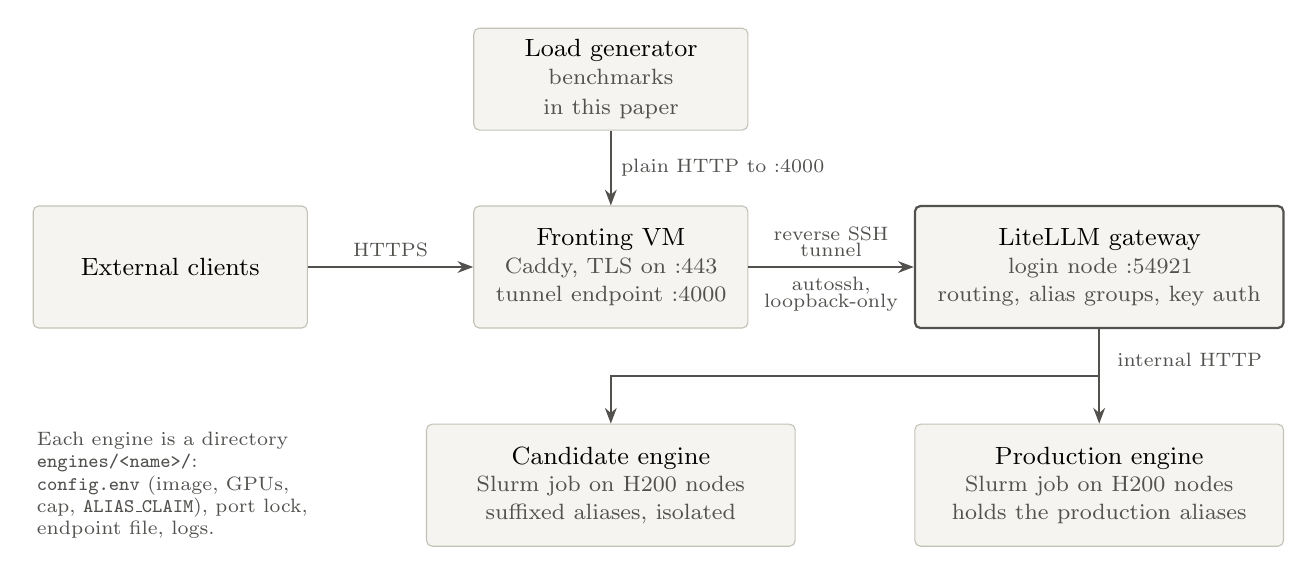
\begin{tikzpicture}[
  font=\small,
  box/.style={draw=axisc, fill=panel, rounded corners=2pt, align=center, inner sep=4pt,
              text width=3.2cm, minimum height=1.55cm,
              execute at begin node={\hyphenpenalty=10000\exhyphenpenalty=10000}},
  gw/.style={box, draw=inksec, line width=0.8pt, text width=4.4cm},
  flow/.style={-{Stealth[length=2mm]}, line width=0.7pt, draw=inksec},
  lab/.style={font=\scriptsize, text=inksec, align=center}]
\node[box] (cli) {External clients};
\node[box, right=2.1cm of cli] (vm) {Fronting VM\\[-1pt]\figsub{Caddy, TLS on :443}\\[-1pt]\figsub{tunnel endpoint :4000}};
\node[box, minimum height=0.9cm, above=0.95cm of vm] (lg) {Load generator\\[-1pt]\figsub{benchmarks in this paper}};
\node[gw, right=2.1cm of vm] (gw) {LiteLLM gateway\\[-1pt]\figsub{login node :54921}\\[-1pt]\figsub{routing, alias groups, key auth}};
\node[box, text width=4.4cm, below=1.2cm of gw] (prod) {Production engine\\[-1pt]\figsub{Slurm job on H200 nodes}\\[-1pt]\figsub{holds the production aliases}};
\node[box, text width=4.4cm] (cand) at (vm |- prod) {Candidate engine\\[-1pt]\figsub{Slurm job on H200 nodes}\\[-1pt]\figsub{suffixed aliases, isolated}};
\node[align=flush left, font=\scriptsize, text=inksec, text width=3.4cm, anchor=west,
      execute at begin node={\hyphenpenalty=10000\exhyphenpenalty=10000}] (note) at ([xshift=-2pt]cli.west |- prod)
  {Each engine is a directory \texttt{engines/<name>/}: \texttt{config.env} (image, GPUs, cap, \texttt{ALIAS\_CLAIM}), port lock, endpoint file, logs.};
\draw[flow] (cli) -- node[lab, above] {HTTPS} (vm);
\draw[flow] (lg) -- node[lab, right] {plain HTTP to :4000} (vm);
\draw[flow] (vm) -- node[lab, above] {reverse SSH\\[-2pt]tunnel} node[lab, below] {autossh,\\[-2pt]loopback-only} (gw);
\coordinate (bus) at ($(gw.south)!0.5!(prod.north)$);
\draw[line width=0.7pt, draw=inksec] (gw.south) -- (bus);
\draw[flow] (bus) -- (prod.north);
\draw[flow] (bus) -| (cand.north);
\node[lab, anchor=south west] at ([xshift=3pt]bus) {internal HTTP};
\end{tikzpicture}
\caption{Request path from external clients through the gateway to engine jobs. A candidate engine registers only suffixed aliases, so it receives benchmark traffic without claiming production names; switching which engine holds the production aliases is a two-line \texttt{ALIAS\_CLAIM} edit plus a gateway restart (Section~\ref{sec:platform}). The benchmarks in this paper entered at the tunnel's plain-HTTP endpoint on the VM, so they exercised the tunnel, gateway, and engines but not the TLS front end.}
\label{fig:arch}
\end{figure}

\begin{table}[t]
\centering
\small
\begin{tabularx}{\textwidth}{lXX}
\toprule
\textbf{Component} & \textbf{Implementation} & \textbf{Notes} \\
\midrule
Gateway & LiteLLM proxy, login node, port 54921 & 5.2\% CPU / 333 MB (observed during the 1,000-user load test) \\
Authentication & Master key + per-user virtual keys (\texttt{key\_tool.py}) & JSON key store with flock and atomic writes; no database; optional per-key RPM/TPM limits enforced in memory \\
Engine lifecycle & \texttt{start\_models.sh} / \texttt{stop\_models.sh} over Slurm & Idempotent dispatch, port locks, endpoint readiness files, two-stage validation (\texttt{validate\_engine.sh}) \\
Routing config & \texttt{generate\_runtime\_config.py} & Static portal models + live probing of engine endpoints; alias groups with production/isolated claims \\
Traffic switching & \texttt{ALIAS\_CLAIM} in each engine's \texttt{config.env} & Production alias set vs.\ suffixed aliases; switching frameworks = edit two lines + gateway restart ($\sim$10 s), engines keep running \\
Container images & Versioned Apptainer SIF files (\texttt{sglang\_0.5.20.sif}, \texttt{vllm\_0.29.1rc1.sif}, dedicated \texttt{vllm\_glm53-flash.sif}) & Version-named; the pull script refuses to overwrite an existing SIF unless forced; dedicated vendor builds used when a model requires them \\
External access & Caddy TLS + autossh reverse tunnel, plus SSH tunnel and web-proxy paths & Loopback-only tunnel binding; IP allowlists at the fronting VM \\
\bottomrule
\end{tabularx}
\caption{Platform components.}
\label{tab:components}
\end{table}

Three design decisions deserve emphasis because they made the A/B protocol of Section~4 cheap to run and safe for production traffic. \emph{First}, engines are self-contained directories (\texttt{engines/<name>/}) whose \texttt{config.env} declares the container image, model path, port, GPU topology, concurrency cap, speculative-decoding settings, and alias claims; starting, stopping, and validating an engine is a single command each, and each engine runs as a separate Slurm job, providing job-level resource isolation. \emph{Second}, the gateway's routing configuration is generated from the \emph{live} set of engine endpoints, so bringing a candidate engine up under suffixed aliases lets it receive production-shaped traffic for validation without claiming the production names; promoting it (or rolling back) is a two-line configuration edit and a ten-second gateway restart. \emph{Third}, container images are version-named SIF files that the pull script refuses to overwrite by default, with a policy of using a vendor's \emph{dedicated} build when one exists for a given model; this policy was validated during the study when a generic nightly vLLM build failed on the KDA model (kernel assertion plus an autotuning hang) while the dedicated build ran correctly (Section~\ref{sec:kda}).

\textbf{Evaluation automation: skills and the agent.} The A/B protocol of Section~4 is not a manual runbook. It is encoded as declarative, versioned procedures---\emph{skills}, in the sense of composable packages of instructions and resources that agents load on demand~\cite{xu2026agentskills}---which an LLM-based coding agent with shell access executes under human approval. Three skills carry the methodology. The \emph{model-onboarding} skill governs how any new model enters the platform: it is official-documentation-first (the agent must locate the vendor's per-model Cookbook or Recipe pages and derive engine flags from them, rather than inventing configurations), recommends dual-framework deployment whenever both frameworks support a model, and encodes the image-version decision flow (versioned names, dedicated builds preferred, ``once supported $\ne$ always supported''). The \emph{concurrency-troubleshooting} skill encodes the layered diagnosis of Section~\ref{sec:reliability} as a symptom$\rightarrow$cause$\rightarrow$fix table, and the \emph{debug-journaling} skill requires that every failure and fix be recorded with its evidence. The repeated A/B measurements of Section~5 are driven by a versioned orchestration script (\texttt{benchmarks/repeats/}) that instantiates isolated engine copies, interleaves the bursts, and collects the evidence of every run. All procedures are included in the artifact repository, making the procedure itself a citable artifact rather than prose. Table~\ref{tab:labor} summarizes the division of labor: the agent performs the mechanical chain, while humans retain the decisions (which model to onboard, which framework releases to pin, and how to weigh verdicts).

\begin{table}[t]
\centering
\small
\begin{tabularx}{\textwidth}{Xcc}
\toprule
\textbf{Pipeline stage} & \textbf{Agent-executed} & \textbf{Human decision} \\
\midrule
Locate official per-model documentation & $\checkmark$ & --- \\
Scaffold + validate both frameworks' engines & $\checkmark$ & Framework releases to pin \\
Deploy under traffic-isolated aliases & $\checkmark$ & --- \\
Run repeated paired benchmark & $\checkmark$ & Workload shape \\
Record verdict (validated-configuration registry) & $\checkmark$ & Interpretation \\
Switch production traffic / roll back & $\checkmark$ & Go/no-go \\
Failure diagnosis during any stage & $\checkmark$ (from encoded symptom$\rightarrow$cause procedures) & --- \\
\bottomrule
\end{tabularx}
\caption{Division of labor in the agent-assisted evaluation workflow. Skills and the orchestration script are version-controlled artifacts of the repository; re-running a decision still requires the same models, images, and hardware.}
\label{tab:labor}
\end{table}

\section{Methodology}
\label{sec:method}

The evaluation asked two questions per model: (i) which framework serves it faster under a high-concurrency burst, and (ii) how enabling the checkpoint's speculative-decoding head changes the absolute throughput. We answer both with paired A/B measurements whose conditions are summarized in Table~\ref{tab:conditions}. The procedure was executed by the LLM-based agent described in Section~\ref{sec:platform}; the human authors made the release decisions (which model, which framework versions to pin) and accepted or rejected verdicts. Every engine flag is traceable to the official documentation the skill requires the agent to cite, and every run's statistics are machine-recorded.

\begin{table}[t]
\centering
\footnotesize
\begin{tabularx}{\textwidth}{l>{\raggedright\arraybackslash}X>{\raggedright\arraybackslash}X>{\raggedright\arraybackslash}X}
\toprule
\textbf{Condition} & \textbf{Dense comparison} & \textbf{Ultra-sparse MoE comparison} & \textbf{KDA comparison} \\
\midrule
Model (same checkpoint both frameworks) & Qwen3.8-27B (BF16, 52 GB) & Qwen3.8-Flash-Next (FP8, 173 GB; 180B/6B active) & GLM-5.3-Flash (FP8, 306 GB) \\
Architecture & Dense hybrid: GDN + full attention & Ultra-sparse MoE: 512 experts + 51B N-gram embedding & KDA linear attention + DSA, 288-expert MoE (8 active), 1M context \\
GPUs per engine & 1$\times$ H200 & 4$\times$ H200 (TP4+EP4) & 8$\times$ H200 (TP8+EP8 / TEP8) \\
Frameworks & SGLang 0.5.20 vs vLLM 0.29.1rc1 & SGLang 0.5.20 vs vLLM 0.29.1rc1 & SGLang 0.5.20 vs vLLM 0.28.1rc1 (dedicated GLM build) \\
Engine parameters & Official docs: SGLang Cookbook vs vLLM Recipe (per-architecture pages) & idem; \texttt{-{}-max-num-seqs 256} per Recipe; SGLang cap aligned to 256; N-gram embedding on GPU for both & idem; BF16 KV cache (FP8 KV unsupported on Hopper for this model, per Recipe) \\
Concurrency cap & 128 both sides (SGLang with EAGLE: 48; Section~\ref{sec:dense}) & 256 both sides & 128 both sides \\
Workload & 500 concurrent requests $\times$ max\_tokens 500 & 1,000 $\times$ 800 & 1,000 $\times$ 800 \\
Output tokens per R1 run & 207k--209k & 514k--528k & 730k--735k \\
Repetitions & 5 interleaved bursts per configuration & 5 & 5, plus 3 further instance pairs (R1) \\
\bottomrule
\end{tabularx}
\caption{A/B conditions. ``R1'' denotes the plain configuration (no speculative decoding); ``R2'' denotes speculative decoding enabled (the checkpoint's integrated MTP/NEXTN head, with each framework's recommended step/top-k settings). Architecture classes: \texttt{Qwen3\_5ForConditionalGeneration} (dense), \texttt{Qwen4ExpForConditionalGeneration} (ultra-sparse MoE), \texttt{Glm5NextForConditionalGeneration} (KDA hybrid). TP/EP: tensor/expert parallelism; TEP: combined tensor--expert parallelism.}
\label{tab:conditions}
\end{table}

\textbf{Repeated-measurement protocol.} For each model and round, both frameworks' engines were started as isolated copies (suffixed aliases, no production traffic) and kept online together, and each configuration was measured in five bursts. The bursts alternated between the two engines, and the leading framework was swapped on every repetition (SGLang first on odd, vLLM first on even), to reduce confounding by drift and run order; the observed difference between a framework's first- and second-position runs was at most about 5.2\%, well below the framework gaps. Each engine received a warm-up of 64 concurrent requests (max\_tokens 64) before measurement, excluded from the statistics, and consecutive bursts were separated by a 60 s cooldown. One exception: a dense vLLM repetition that was re-run on a fresh engine instance after a client-side failure did not receive the warm-up (Section~\ref{sec:dense}). Two controls isolate confounds identified during the study: a cap-48 plain configuration for the dense model (Section~\ref{sec:dense}) and a 600 s client deadline for the KDA R2 round (Section~\ref{sec:kda}). All repeated measurements were taken on 2026-09-28/29; the original single runs of 2026-09-27, taken without warm-up, are reported alongside for comparison. Protocol deviations and their causes (for example, excluded nodes) are logged in the run manifest.

\textbf{Fairness controls.} Each pair of runs used (a) the same local checkpoint directory (bit-identical weights, no downloads), (b) the same GPU type, with both engines online in the same time window, (c) concurrency caps set equal on both sides, except where a framework cannot start at the shared cap (SGLang with EAGLE on the dense model; Section~\ref{sec:dense}), and (d) engine startup parameters derived from each framework's official per-model documentation, with the experimental overrides recorded in the condition files (cap alignment, speculative-decoding settings, and SGLang's Mamba-cache size of cap $\times$ 5). Output tokens per R1 run stayed within $\pm$1.7\% of each model's mean across frameworks and repetitions (Table~\ref{tab:conditions}); R2 runs truncated by the client deadline are excluded from this check, which in any case does not establish equal per-request work or equal output quality. Across all repeated runs, eleven requests were lost to transport-level connection resets about 1.5 s after submission, before any response; they count as not completed. The client harness, an httpx-based load generator (\texttt{stress\_test.py}), drives a fixed pool of five short technical-QA prompts (cycled across requests at temperature 0.7) from the fronting VM through the reverse tunnel and the gateway to the engine, and records per-request latency, token counts, finish reason, and an output fingerprint. The client uses a 300 s request deadline, set earlier from the longest request observed on this platform (188 s) plus margin rather than from a service-level objective. The benchmark key carries no rate limit, and the gateway's upstream timeout (600 s) exceeds the client deadline.

\textbf{Metrics.} We report \emph{aggregate} throughput (total output tokens divided by wall time) as mean $\pm$ sample standard deviation over repetitions, the per-repetition paired SGLang/vLLM throughput ratio, \emph{completion rate} (requests completed within the client deadline $\div$ total), and \emph{tail latency} (P95). Because every burst releases all requests at once, P95 largely reflects queue-drain time rather than per-request service latency.

\section{Results}

\subsection{Dense hybrid: SGLang +9.6\%}
\label{sec:dense}

On the 27B dense hybrid, SGLang led by 9.6\% on average and in every paired repetition (Table~\ref{tab:dense-r1}); the paired SGLang/vLLM ratio was $1.097 \pm 0.026$ (range 1.071--1.139).

\begin{table}[t]
\centering
\begin{tabular}{lcc}
\toprule
\textbf{Metric} & \textbf{SGLang 0.5.20 (R1)} & \textbf{vLLM 0.29.1rc1 (R1)} \\
\midrule
Aggregate throughput ($n=5$) & \textbf{3,882 $\pm$ 36 \tps} & 3,541 $\pm$ 95 \tps \\
P95 latency & \textbf{50.9 $\pm$ 0.4 s} & 55.9 $\pm$ 1.6 s \\
Completion rate & 100\% (all runs) & 100\% (all runs) \\
Original single run (2026-09-27) & 3,823 \tps & 3,597 \tps \\
\bottomrule
\end{tabular}
\caption{Dense comparison, R1 (plain). One vLLM repetition was re-run on a fresh engine instance after a client-side failure and, unlike the others, without the client warm-up; it measured 3,372 \tps, 5.9\% below the other four, and accounts for most of the vLLM spread. The rerun was not part of the original back-to-back pairing; excluding it, the other four pairs give vLLM $3{,}584 \pm 13$ \tps{} and a paired ratio of $1.086 \pm 0.011$, and SGLang still led in every repetition.}
\label{tab:dense-r1}
\end{table}

Enabling the checkpoint's integrated draft head cost both frameworks throughput, but for different reasons (Table~\ref{tab:dense-r2}). vLLM's MTP shares weights with the target model and kept cap 128; it lost 6.7\%. SGLang's EAGLE loads draft weights plus an intermediate-state cache for the GDN blocks (13.8 GB at cap 48, 22.8 GB at cap 80), and with it SGLang cannot allocate KV cache for 128 concurrent requests on one H200: in our sweep, caps of 96, 112, and 128 failed at startup and 80 started (caps 81--95 were not tested); SGLang's own automatic setting is 48. The original study's configuration set cap 48 explicitly, with a Mamba cache of 240 (48 $\times$ 5); at that configuration SGLang lost 39.5\% against its plain cap-128 configuration. A cap-48 plain control separates the two effects: lowering the cap from 128 to 48 alone costs 47.3\% (vLLM: 45.9\%), while EAGLE at equal cap \emph{raises} throughput by 14.8\%. Even at the highest tested feasible cap (80), SGLang with EAGLE remained 34.1\% below its plain configuration.

\begin{table}[t]
\centering
\small
\begin{tabular}{lcc}
\toprule
\textbf{Configuration} & \textbf{SGLang 0.5.20} & \textbf{vLLM 0.29.1rc1} \\
\midrule
R1 plain, cap 128 & \textbf{3,882 $\pm$ 36} & 3,541 $\pm$ 95 \\
Plain, cap 48 (control) & 2,046 $\pm$ 11 & 1,917 $\pm$ 24 \\
R2 speculative, cap 48 (SGLang) / 128 (vLLM) & 2,348 $\pm$ 10 (\textbf{$-$39.5\%}) & 3,304 $\pm$ 22 (\textbf{$-$6.7\%}) \\
R2 speculative, cap 80 (highest tested feasible) & 2,559 $\pm$ 14 (\textbf{$-$34.1\%}) & --- \\
\bottomrule
\end{tabular}
\caption{Dense comparison, speculative decoding and concurrency (\tps, $n=5$; percentages relative to the same framework's R1). SGLang uses EAGLE 3/1/4 (steps/draft/tokens); vLLM uses MTP$\times$3. In the cap-48 plain control, the SGLang/vLLM ratio is $1.067 \pm 0.015$, the same direction as R1.}
\label{tab:dense-r2}
\end{table}

\subsection{\texorpdfstring{Ultra-sparse MoE: vLLM 2.40$\times$}{Ultra-sparse MoE: vLLM 2.40x}}
\label{sec:moe}

On the ultra-sparse MoE, the ranking reversed (Table~\ref{tab:moe}): the paired SGLang/vLLM ratio was $0.417 \pm 0.014$, so vLLM delivered 2.40$\times$ the throughput of SGLang, and 2.02$\times$ that of SGLang's best configuration.

\begin{table}[t]
\centering
\small
\begin{tabular}{lcc}
\toprule
\textbf{Configuration} & \textbf{SGLang 0.5.20} & \textbf{vLLM 0.29.1rc1} \\
\midrule
R1 aggregate throughput & 3,299 $\pm$ 82 & \textbf{7,921 $\pm$ 124} \\
R1 P95 latency & 153.1 $\pm$ 3.8 s & \textbf{63.2 $\pm$ 1.1 s} \\
R2 (speculative) & 3,930 $\pm$ 117 (NEXTN, \textbf{+19.1\%})$^{a}$ & 4,394 $\pm$ 138 (MTP$\times$3, \textbf{$-$44.5\%}) \\
Best per framework & 3,930 (NEXTN on) & \textbf{7,921 (plain)} \\
Original single run, R1 & 3,383 & 7,886 \\
\bottomrule
\end{tabular}
\caption{Ultra-sparse MoE comparison (\tps, $n=5$). $^{a}$One repetition completed 99.8\% of requests (two connections reset about 1.5 s after submission, before any response); all other runs completed 100\%. Both frameworks keep the 51B N-gram embedding on GPU; in the original single-run study, SGLang's default CPU offload of the embedding was 2.6\% slower.}
\label{tab:moe}
\end{table}

The same integrated draft head moved the two frameworks in opposite directions: SGLang's NEXTN gained 19.1\%---consistent with the model's low 6B-active decode cost making draft-and-verify cheap---while vLLM's MTP lost 44.5\%, matching the vendor recipe's warning against enabling it by default on this architecture. We attribute the R1 gap to MoE execution---vLLM's Triton MoE and FP8 pipeline for this architecture appeared more mature in the versions tested---although we did not profile kernels to confirm the attribution.

\subsection{KDA hybrid: vLLM +28\%}
\label{sec:kda}

On the KDA model, vLLM led (Table~\ref{tab:kda}): the paired SGLang/vLLM ratio was $0.782 \pm 0.037$, and three further pairs of freshly started engine instances gave 0.757, 0.768, and 0.763 (all four pairs, weighted equally although the main pair has $n=5$ and the others $n=2$: $0.767 \pm 0.010$, i.e.\ vLLM +30\%). All four pairs favored vLLM, and the cross-instance CV of the instance-mean throughput was 1.0\% for SGLang and 2.0\% for vLLM. The vLLM side requires a \emph{dedicated} vendor build (0.28.1rc1 with precompiled GLM kernels); the generic nightly build failed during startup with a kernel assertion and a 31-minute autotuning hang, an observation that motivated our image-governance policy of preferring dedicated builds when they exist.

\begin{table}[t]
\centering
\small
\begin{tabular}{lcc}
\toprule
\textbf{Configuration} & \textbf{SGLang 0.5.20} & \textbf{vLLM 0.28.1rc1 (dedicated)} \\
\midrule
R1 aggregate throughput & 3,687 $\pm$ 71 & \textbf{4,719 $\pm$ 201} \\
R1 P95 latency & 193.5 $\pm$ 3.7 s & \textbf{150.3 $\pm$ 6.9 s} \\
R2 (speculative), 300 s client deadline & \textbf{3,362 $\pm$ 60} (\textbf{$-$8.8\%}) & 2,328 $\pm$ 108, censored$^{a}$ \\
R2 (speculative), 600 s client deadline & \textbf{3,251 $\pm$ 68} & 2,420 $\pm$ 11$^{b}$ (\textbf{$-$48.7\%}) \\
Best per framework & 3,687 (plain) & \textbf{4,719 (plain)} \\
Original single run, R1 & 3,669 & 2,857 \\
\bottomrule
\end{tabular}
\caption{KDA comparison (\tps, $n=5$; percentages relative to the same framework's R1). R2 uses SGLang EAGLE 5/1/6 and vLLM MTP$\times$5; the two R2 rounds ran on different engine instances. $^{a}$0--10.5\% of requests per repetition were not completed within the 300 s deadline, so throughput counts completed requests only. $^{b}$No request reached the deadline; 4,997 of 5,000 requests completed, the other three lost in one repetition to connection resets about 1.5 s after submission.}
\label{tab:kda}
\end{table}

\textbf{A single run reversed this ranking.} The original single run, taken without warm-up, placed SGLang first by 28\% and understated vLLM by 39\% (2,857 vs.\ $4{,}719 \pm 201$ \tps). Its engine log shows runtime compilation of TileLang kernels in the middle of the measured burst---nine compilation events logged by rank~0 in R1, and three per rank in R2---with generation throughput falling to 10--20 \tps{} while they ran. In the repeated protocol, the runtime-JIT warnings that vLLM's monitor emits for this model appeared during the warm-up and never in a measured burst. A single-factor control, in which each engine started with an empty TileLang cache and ran one burst without warm-up followed by a second, confirmed that these runtime-JIT warnings occur only in the first burst, but did not isolate their throughput cost, and it did not reproduce the original cache state (with an empty cache, this build precompiles its TileLang kernels at startup): across three repetitions the first burst was not consistently slower, and one node showed generation stalls unrelated to JIT. We therefore attribute the original error to single-run measurement without warm-up---runtime compilation and instance-level stalls both distort a single burst---rather than to JIT alone.

\textbf{Speculative decoding and the client deadline.} Speculative decoding lowered throughput on both frameworks. On vLLM it also pushed the burst's queue-drain time past the client's 300 s deadline: 0--10.5\% of requests were abandoned by the client in individual repetitions, although the engine reported no errors. With a 600 s deadline, no request timed out (the slowest took 305 s); 4,997 of 5,000 requests completed, the other three lost to early transport-level connection resets, and vLLM's R2 throughput, no longer deadline-censored, was $2{,}420 \pm 11$ \tps, 48.7\% below its plain configuration. The operational consequence was immediate: our production SGLang deployment had been running with MTP enabled, and disabling it---a change shipped the same day by editing the engine's \texttt{config.env}---raises throughput by 9.7\% in the repeated measurements. Under this workload vLLM would serve GLM-5.3-Flash 28\% faster still; production has not been switched.

\subsection{Cross-architecture synthesis}
\label{sec:synthesis}

Table~\ref{tab:synthesis} and Figure~\ref{fig:throughput} collect the headline results: the leading framework depended on the architecture, and the margin ranged from 9.6\% to 2.40$\times$.

\begin{figure}[t]
\centering
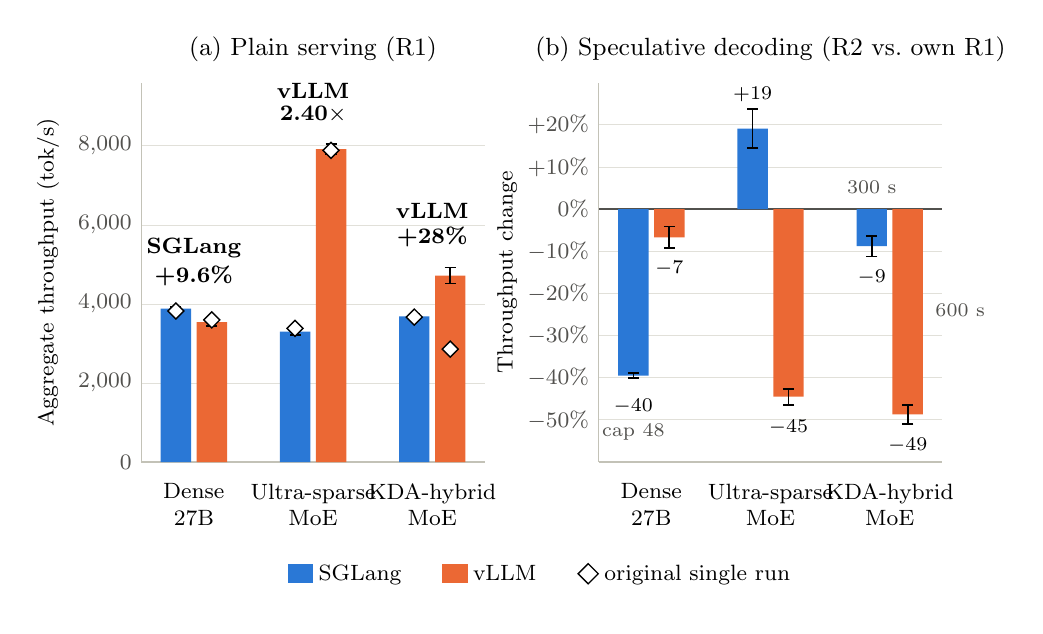
\begin{tikzpicture}
\begin{groupplot}[
  group style={group size=2 by 1, horizontal sep=1.45cm},
  width=0.49\textwidth, height=6.4cm,
  ybar, /pgf/bar width=11pt,
  symbolic x coords={Dense,MoE,KDA},
  xtick=data,
  xticklabels={{Dense\\27B},{Ultra-sparse\\MoE},{KDA-hybrid\\MoE}},
  xticklabel style={align=center, font=\footnotesize, text=black},
  enlarge x limits=0.22,
  axis lines*=left, axis line style={draw=axisc}, tick style={draw=none},
  ymajorgrids=true, grid style={draw=gridc, line width=0.3pt},
  yticklabel style={font=\footnotesize, text=inksec},
  ylabel style={font=\footnotesize},
  title style={font=\small, yshift=-2pt},
  legend style={draw=none, font=\footnotesize, legend columns=3,
                /tikz/every even column/.append style={column sep=0.45cm}},
  legend image code/.code={\draw[#1, draw=none] (0cm,-0.1cm) rectangle (0.32cm,0.14cm);},
  error bars/error bar style={line width=0.6pt, draw=black},
  error bars/error mark options={rotate=90, mark size=2pt, line width=0.6pt, draw=black},
]
% (a) R1 throughput, mean +- SD over five repetitions; open diamonds = original single runs
\nextgroupplot[title={(a) Plain serving (R1)},
  ymin=0, ymax=9600, ytick={0,2000,4000,6000,8000}, yticklabels={0,2{,}000,4{,}000,6{,}000,8{,}000},
  clip=false,
  ylabel={Aggregate throughput (\tps)},
  legend to name=fwlegend]
\addplot[fill=sglang, draw=none, bar shift=-6.5pt, error bars/.cd, y dir=both, y explicit]
  coordinates {(Dense,3882) +- (0,36) (MoE,3299) +- (0,82) (KDA,3687) +- (0,71)};
\addlegendentry{SGLang}
\addplot[fill=vllm, draw=none, bar shift=6.5pt, error bars/.cd, y dir=both, y explicit]
  coordinates {(Dense,3541) +- (0,95) (MoE,7921) +- (0,124) (KDA,4719) +- (0,201)};
\addlegendentry{vLLM}
\addlegendimage{legend image code/.code={\node[draw=black, fill=white, diamond, inner sep=1.5pt, line width=0.5pt] at (0.16cm,0.02cm) {};}}
\addlegendentry{original single run}
\foreach \x/\y in {Dense/3823, MoE/3383, KDA/3669}
  {\edef\tmp{\noexpand\node[draw=black, fill=white, diamond, inner sep=1.5pt, line width=0.5pt] at ([xshift=-6.5pt]axis cs:\x,\y) {};}\tmp}
\foreach \x/\y in {Dense/3597, MoE/7886, KDA/2857}
  {\edef\tmp{\noexpand\node[draw=black, fill=white, diamond, inner sep=1.5pt, line width=0.5pt] at ([xshift=6.5pt]axis cs:\x,\y) {};}\tmp}
\node[font=\footnotesize\bfseries, anchor=south] at (axis cs:Dense,3918) [yshift=4pt] {\shortstack{SGLang\\+9.6\%}};
\node[font=\footnotesize\bfseries, anchor=south] at (axis cs:MoE,8045) [yshift=4pt] {\shortstack{vLLM\\2.40$\times$}};
\node[font=\footnotesize\bfseries, anchor=south] at (axis cs:KDA,4920) [yshift=4pt] {\shortstack{vLLM\\+28\%}};
% (b) effect of speculative decoding, relative to the same framework's R1, mean +- SD
\nextgroupplot[title={(b) Speculative decoding (R2 vs.\ own R1)},
  ymin=-60, ymax=30, ytick={-50,-40,-30,-20,-10,0,10,20},
  yticklabels={$-50\%$,$-40\%$,$-30\%$,$-20\%$,$-10\%$,0\%,$+10\%$,$+20\%$},
  ylabel={Throughput change}, ylabel shift=-3pt, clip=false,
  extra y ticks={0}, extra y tick labels={},
  extra y tick style={grid style={draw=inksec, line width=0.6pt}}]
\addplot[fill=sglang, draw=none, bar shift=-6.5pt, error bars/.cd, y dir=both, y explicit]
  coordinates {(Dense,-39.5) +- (0,0.6) (MoE,19.1) +- (0,4.6) (KDA,-8.8) +- (0,2.4)};
\addplot[fill=vllm, draw=none, bar shift=6.5pt, error bars/.cd, y dir=both, y explicit]
  coordinates {(Dense,-6.7) +- (0,2.6) (MoE,-44.5) +- (0,1.9) (KDA,-48.7) +- (0,2.2)};
\foreach \x/\y/\l/\s in {Dense/-39.5/$-$40/-6.5pt, MoE/19.1/+19/-6.5pt, KDA/-8.8/$-$9/-6.5pt, Dense/-6.7/$-$7/6.5pt, MoE/-44.5/$-$45/6.5pt, KDA/-48.7/$-$49/6.5pt}
  {\edef\tmp{\noexpand\node[font=\noexpand\scriptsize, anchor=\ifdim\y pt<0pt north\else south\fi] at ([xshift=\s]axis cs:\x,\y) [yshift=\ifdim\y pt<0pt -5pt\else 6pt\fi] {\l};}\tmp}
\node[font=\scriptsize, text=inksec, anchor=north, align=center] at ([xshift=-6.5pt]axis cs:Dense,-39.5) [yshift=-14pt] {cap 48};
\node[font=\scriptsize, text=inksec, anchor=south] at ([xshift=-6.5pt]axis cs:KDA,0) [yshift=2pt] {300 s};
\node[font=\scriptsize, text=inksec, anchor=west] at ([xshift=13pt]axis cs:KDA,-24) {600 s};
\end{groupplot}
\node[anchor=north] at ($(group c1r1.south)!0.5!(group c2r1.south)+(0,-1.05cm)$) {\pgfplotslegendfromname{fwlegend}};
\end{tikzpicture}
\caption{The three comparisons at a glance (values from Tables~\ref{tab:dense-r1}--\ref{tab:kda}). (a)~Plain-serving throughput, mean $\pm$ SD over five repetitions; the label above each pair names the leader and its margin, and open diamonds mark the original single runs, of which the KDA vLLM run understated throughput by 39\% and reversed the ranking. (b)~Change in aggregate throughput when the checkpoint's speculative-decoding head is enabled, as the ratio of mean throughputs $r = \bar{m}_{R2}/\bar{m}_{R1}$ minus one; error bars propagate the two standard deviations, $100\,r\sqrt{(s_{R2}/\bar{m}_{R2})^2 + (s_{R1}/\bar{m}_{R1})^2}$, ignoring covariance, and are not standard errors or confidence intervals. Five of six bars are below zero. SGLang's dense bar is at its EAGLE cap of 48 (Section~\ref{sec:dense}); for KDA, SGLang is from the 300 s round and vLLM from the 600 s round, on different engine instances (Section~\ref{sec:kda}).}
\label{fig:throughput}
\end{figure}

\begin{table}[t]
\centering
\small
\begin{tabular}{llr@{\hspace{1.4em}}cc}
\toprule
 & & & \multicolumn{2}{c}{\textbf{R2 vs.\ own R1}} \\
\cmidrule(l){4-5}
\textbf{Architecture (model)} & \textbf{R1 leader} & \textbf{Margin ($n=5$)} & \textbf{SGLang} & \textbf{vLLM} \\
\midrule
Dense hybrid (Qwen3.8-27B) & SGLang & +9.6\% & $-$39.5\%$^{a}$ & $-$6.7\% \\
Ultra-sparse MoE (Qwen3.8-Flash-Next) & vLLM & 2.40$\times$ & +19.1\% & $-$44.5\% \\
KDA-hybrid MoE (GLM-5.3-Flash) & vLLM & +28\% & $-$8.8\%$^{b}$ & $-$48.7\%$^{c}$ \\
\bottomrule
\end{tabular}
\caption{Synthesis across the three comparisons. $^{a}$At SGLang's EAGLE cap of 48; at equal cap EAGLE gains 14.8\%, and at the highest tested feasible cap (80) the loss is 34.1\% (Section~\ref{sec:dense}). $^{b}$300 s round, in which no SGLang request approached the deadline. $^{c}$600 s round, which removes the truncation of the 300 s round (Section~\ref{sec:kda}). Each framework uses its documented speculative settings; the five-negative, one-positive pattern holds for either dense SGLang cap (48 or 80) and either KDA deadline round. Framework versions as in Table~\ref{tab:conditions}.}
\label{tab:synthesis}
\end{table}

Two regularities stand out. First (Figure~\ref{fig:throughput}a), the framework gap was smallest on the well-trodden dense hybrid (9.6\%) and largest on the newer ultra-sparse MoE (2.4$\times$), which may reflect how recently each framework acquired mature kernels for a given architecture---though with one model per architecture we cannot separate this from framework-version and workload differences. Second (Figure~\ref{fig:throughput}b), speculative decoding lowered throughput in five of the six framework--model pairs in their deployable configurations. For vLLM on all three models and SGLang on the KDA model, the loss is consistent with draft-and-verify work competing with decode batches that already occupy the GPU, although we did not profile it; for SGLang on the dense model it is a memory effect (Section~\ref{sec:dense}); and the single gain (SGLang NEXTN on the 6B-active MoE) is consistent with cheap decodes leaving headroom for drafting.

\subsection{Platform-level capacity and reliability}
\label{sec:reliability}

Beyond per-engine comparisons, the platform sustained a mixed workload of 1,500 concurrent users across all three engines with 100\% success, 8,146 \tps{} aggregate throughput, and 76.8 s P95 from the fronting VM through the tunnel and gateway (Table~\ref{tab:reliability}). Gateway overhead at this load was 2.5\% CPU and 405 MB of memory, and no gateway-related failures were observed at the tested burst size. The measurements in this section are single runs, and the gateway CPU and memory figures here and in Table~\ref{tab:components} are observations recorded in the operations log at the time rather than retained telemetry.

\begin{table}[t]
\centering
\footnotesize
\begin{tabularx}{\textwidth}{>{\raggedright\arraybackslash}Xccc>{\raggedright\arraybackslash}p{4.9cm}}
\toprule
\textbf{Stage of the reliability investigation} & \textbf{Success} & \textbf{Aggregate} & \textbf{P95} & \textbf{Root cause identified} \\
\midrule
Initial mixed run (1,500 users) & 67.9\% & --- & --- & Client shell \texttt{ulimit -n} 1024 $\rightarrow$ fd exhaustion (Errno 24) at $\sim$1,020 open sockets \\
After client fix, via tunnel & 91.8\% & 8,251 \tps & 70.4 s & Per-connection sshd on the tunnel VM also capped at 1024 fds (verified via \texttt{/proc/<pid>/limits}) \\
Bypassing the tunnel (direct) & 100\% & 8,156 \tps & 77.6 s & Isolated remaining losses to the VM$\leftrightarrow$gateway segment \\
After \texttt{/etc/security/limits.conf} fix, via tunnel & \textbf{100\%} & 8,146 \tps & 76.8 s & Correct fix: PAM \texttt{limits.conf} (systemd override alone does not apply to per-connection sshd); tunnel re-established after the fix \\
\bottomrule
\end{tabularx}
\caption{Layered attribution of mixed-load failures (1,500 users $\times$ 500 tokens; three engines live).}
\label{tab:reliability}
\end{table}

We report this debugging arc as a result in its own right for two reasons. First, an initial hypothesis---that an 8\% ReadError rate indicated a single-flow ceiling of the reverse tunnel---was \emph{refuted} by the fix-and-remeasure cycle: after correcting both fd limits, 1,500 concurrent users traversed the single tunnel flow at 100\% success, so no such ceiling was reached below 1,500. Second, the diagnosis illustrates a methodology we now apply routinely: measure each layer independently (client $\rightarrow$ tunnel $\rightarrow$ gateway $\rightarrow$ engine), fix one layer at a time, and re-run the identical workload after each fix rather than trusting bypass experiments to localize faults finer than segment granularity.

\section{Discussion}

\textbf{Framework choice is a per-model decision, and it is large.} The observed spread---from a 9.6\% margin to a 2.40$\times$ gap---is the largest lever we measured on correctly configured engines. Concurrency-cap tuning, in separate single-run measurements on the same engines, raised aggregate throughput by 29\% (MoE, cap 48 $\rightarrow$ 100) and 32\% (KDA, cap 64 $\rightarrow$ 128), and restoring a misconfigured SGLang baseline on the dense engine had earlier been worth +48\%. In operational terms, the measured framework gap on the ultra-sparse MoE exceeded the effects of every configuration change we evaluated. The practical implication we adopted institutionally is a \emph{dual-framework onboarding policy}: every new model is deployed on both frameworks under suffixed aliases, A/B-tested under the production workload, and promoted by a two-line configuration change; the platform of Section~\ref{sec:platform} makes this a routine procedure rather than a redeployment project. The results do not favor either framework in general: each led on at least one of the three architectures.

\textbf{Single-run benchmarks can pick the wrong champion.} Our first comparison of the KDA model, a single burst without warm-up, named SGLang the winner by 28\%; five warmed-up, interleaved repetitions and three further engine-instance pairs named vLLM the winner by 28--30\%, with all four instance pairs favoring vLLM. The single run used the same checkpoint, hardware, and documented parameters as the repeated protocol; what it lacked was warm-up and repetition, and on a new architecture whose kernels compile at runtime, one burst can absorb compilation stalls that a steady-state service never sees. Because the orchestration is a versioned artifact, the correction was produced by re-running the procedure rather than by re-engineering the study; we recommend that framework comparisons on new architectures report repeated, warmed-up measurements as a minimum.

\textbf{Speculative decoding at high concurrency.} Our results add same-checkpoint, repeated evidence from a production platform on how speculative decoding behaves under load: with 500--1,000 concurrent requests, enabling the integrated draft head lowered net throughput in five of six pairs. For vLLM on all three models and SGLang on the KDA model this is consistent with the mechanism goodput analyses describe---verification work competing with useful decoding when speculation ignores load~\cite{liu2024turbospec}---although we did not profile it; for SGLang on the dense model the loss is a memory effect (below). Adaptive systems such as TurboSpec address this by gating speculation on measured goodput~\cite{liu2024turbospec}, and AdaServe by customizing it to per-request SLOs~\cite{li2025adaserve}; our measurements suggest a cruder but zero-engineering-cost policy---disable integrated MTP/NEXTN by default for short-prompt, high-concurrency throughput serving of these architectures, and enable it only where a measurement shows a gain, as for SGLang NEXTN on the MoE. We do \emph{not} conclude that speculative decoding is useless: at low concurrency, for single-stream latency, or---per MagicDec's analysis---for long contexts under high batch~\cite{sadhukhan2024magicdec} it can remain appropriate, and the one positive case here (SGLang NEXTN, +19\% at 6B active parameters) is consistent with a model-dependent crossover, as in the goodput formulation~\cite{liu2024turbospec}. The decision should be made from a measurement at the deployment's own concurrency, not from the feature's reputation.

\textbf{Memory accounting can decide speculative feasibility.} On the dense hybrid, the decisive cost of SGLang's EAGLE was not computation but memory: the draft weights and the GDN intermediate-state cache (13.8 GB at cap 48, 22.8 GB at cap 80) made 80 the highest feasible cap we tested on one H200, and the concurrency lost ($-$47\% from 128 to 48) outweighs what drafting gains (+15\% at equal cap). vLLM's MTP shares the head weights within the checkpoint and preserved the cap. On models whose caches dominate memory, this implementation difference can outweigh acceptance-rate considerations, and it is invisible in feature lists; a feasibility sweep of the concurrency cap is a cheap way to expose it.

\textbf{Dedicated builds and version governance.} The KDA comparison could not be run on the generic vLLM nightly at all (kernel assertion; autotuning hang), while the vendor's dedicated build ran correctly. Our resulting policy---version-named images that are not overwritten by default, dedicated builds preferred when they exist, ``once supported $\ne$ always supported''---converted what could have been days of kernel-level debugging into a one-line image selection. Framework \emph{version} is a first-class experimental variable on new architectures, and evaluations that do not pin and report it are hard to reproduce.

\textbf{What the platform measurements do and do not show.} The layered analysis of Section~\ref{sec:reliability} observed no gateway- or tunnel-related failures at the tested burst size: the gateway used 2.5\% CPU at 1,500 users, and no single-flow tunnel ceiling was observed below 1,500 users. These runs did not pass through the TLS front end and include no capacity sweep, so they do not establish where the next bottleneck lies.

\textbf{Agents as experimentalists.} Beyond its findings, this study is a working example of an LLM-based agent assisting with an experimental procedure under human approval. Autonomous research agents have been demonstrated for closed-loop scientific discovery~\cite{lu2024aiscientist}; agent-driven simulation has been proposed to track the fast-moving serving design space because real deployments are costly~\cite{kim2026simthesizer}; and AutoTuneBench has agent systems auto-tune both engines under a strict measurement protocol~\cite{chen2026autotunebench}. Our pipeline is closest to the last of these but different in object: AutoTuneBench tunes engine configurations, whereas our skills drive the full production lifecycle---deployment behind a live gateway, benchmarking through the external traffic path, verdict recording, and production traffic switching---on infrastructure that keeps serving users throughout.

What made the automation trustworthy was not the agent's raw capability but the enclosure: declarative skills that require documentation-traceable configuration, traffic isolation that makes candidate engines harmless to production, versioned orchestration that records every run, and mandatory evidence journaling. Within that enclosure, the agent performed work that would otherwise gate on scarce systems-engineering time---including the repeated measurements and controls of Section~5, which the agent planned, executed, and diagnosed (excluding faulty nodes and correcting a mis-specified condition along the way) under the first author's direction. Related benchmarks evaluate how well agents do DevOps tasks~\cite{tang2026devopsgym}; here the DevOps task itself---deploying, benchmarking, and switching production inference infrastructure---was the experiment. We take this as an operational answer to the question this paper opened with: ``which framework should serve this model?'' is better answered by a repeated measurement whose procedure is a versioned artifact of the repository than by folklore or release notes.

\section{Limitations and Future Work}

Five limitations bound our conclusions. \emph{Workload.} All comparisons use one workload shape---a single burst of short technical-QA prompts at uniform max\_tokens, released at once---so latency percentiles reflect queue drain rather than steady-state service, and results may differ for long contexts, open-loop arrivals, or streaming metrics (time to first token and time per output token), none of which we measured. \emph{Mechanism.} We did not profile kernels, GPU utilization, or speculative acceptance lengths, so the attributions offered for the MoE gap and for the speculative-decoding losses remain hypotheses; the harness records output fingerprints but runs no output-quality evaluation. \emph{Scope.} We test one model per architecture, one GPU type, and single-engine deployments; the MoE gap in particular should be expected to move as kernels mature, the speculative cap sweep did not test caps 81--95, and multi-instance configurations were validated only for success rate (Section~\ref{sec:reliability}). We report an agent-assisted deployment workflow, not a controlled comparison of agent and human effectiveness. \emph{Variance.} Repetitions within an engine instance agreed closely (CV mostly below 3\%), but one dense repetition without warm-up measured 5.9\% below the others; in a KDA control without warm-up, first bursts measured 3,839--4,170 \tps{} and later bursts 2,999--4,622 \tps, the lowest on one node with generation stalls unrelated to JIT; separately, the four warmed-up instance means averaged $4{,}866 \pm 98$ \tps; the concurrency-tuning and reliability numbers of Sections~\ref{sec:reliability} and~6 are single runs. \emph{Provenance.} SHA-256 digests of the container images were recorded for the repeated measurements; the original single runs used images that were later renamed to version-named files, and no digests were recorded for them. Model checkpoints are identified by file listing rather than by revision.

Future work should extend the matrix in five directions: mixed and open-loop workload shapes with streaming TTFT/TPOT; FP8-versus-BF16 and KV-cache-dtype axes, which our Hopper hardware partially constrains for the KDA model (FP8 KV unsupported); later framework releases, to calibrate how quickly such evaluations expire; a concurrency sweep for speculative decoding, recording acceptance lengths; and kernel-level profiling to test the mechanism attributions offered in Section~5.

\section{Conclusion}

We built a multi-model API service on an HPC cluster---a LiteLLM gateway over Slurm-managed engines on H200 GPUs---and, confronted with the recurring question of which serving framework to assign to each new model, encoded the comparison as versioned skills and an orchestration script that an LLM-based agent executes under human approval: scaffold both frameworks from official documentation, deploy them under traffic-isolated aliases, benchmark both in repeated, interleaved, warmed-up bursts, record the verdict, and switch production traffic when warranted. Applied to three architecturally distinct LLMs, the comparisons found that the leading framework depended on the architecture---SGLang +9.6\% on a dense hybrid, vLLM 2.40$\times$ on an ultra-sparse MoE, vLLM +28\% on a KDA-hybrid MoE---and that speculative decoding with integrated draft heads lowered throughput in five of six framework--model pairs, in one case because of memory rather than computation. A single run without warm-up had named the wrong winner for the KDA model. Together, the results argue for treating framework selection and speculative decoding not as defaults to be inherited but as per-model, per-workload decisions---and for making the repeated measurement that informs them cheap and safe enough to run on every new model, which is the purpose of the agent-assisted procedure described here.

\section*{AI-Use Disclosure}

LLM-based coding agents assisted with engine deployment, benchmark orchestration, failure diagnosis, literature searches and reference checks, and manuscript drafting, review, and revision, including figures and LaTeX preparation. The agents operated under human direction using the versioned procedures described in this paper. The tools used were opencode (GLM-5.3), Claude Code (Anthropic Claude Opus 5.5), and GPT-6 (ASTRA). The human authors defined the research questions and methodology, made deployment and release decisions, and retain responsibility for the results, references, and final manuscript.

\section*{Author Contributions}

\textbf{Chao-Chun Chuang:} Conceptualization, Methodology, Software, Investigation, Formal analysis, and Writing --- original draft (AI-assisted, under the author's direction; see AI-Use Disclosure). \textbf{Po-Hsiang Lin:} Investigation, Data curation, Validation, and Writing --- review and editing. \textbf{Liang-Hsun Huang:} Validation (checking the manuscript's descriptions of the models' architectures, parameters, and terminology against their official documentation) and Writing --- review and editing.

\section*{Funding}

\begin{sloppypar}
This work was supported in part by the National Science and Technology Council (NSTC), Taiwan, under Grant Nos.\ NSTC 115-2410-H-A49-046-MY3 and NSTC 114-2634-F-006-002.
\end{sloppypar}

\section*{Competing Interests}

The authors declare that they have no competing interests.

\section*{Acknowledgments}

The authors gratefully acknowledge the National Center for High-performance Computing (NCHC), National Institutes of Applied Research (NIAR), Taiwan, for providing the research resources, computational infrastructure, and platform services that supported this work.

\section*{Data and Artifact Availability}

The artifact repository (release \texttt{v1.0.1})
\begin{center}\url{https://github.com/gemini960114/no-permanent-champion-research-artifact}\end{center}
\noindent provides a curated snapshot of the experimental materials supporting this paper, including raw measurements, analysis scripts, benchmark configurations, and redacted execution logs. The repeated measurements are in \texttt{benchmarks/\allowbreak results/\allowbreak repeats/\allowbreak 20260928-153829/}: per-run summaries and per-request records for every configuration and control, the run manifest and event log, the redacted engine configurations and logs (including, in \texttt{original\_run\_logs/}, the engine logs of the original single runs cited in Section~\ref{sec:kda}), Slurm job records, and the aggregated tables; the original single runs are in \texttt{benchmarks/\allowbreak results/}, and the client-side summary of the initial 67.9\% mixed run (Table~\ref{tab:reliability}) is in \texttt{benchmarks/\allowbreak results/\allowbreak client\_vm/}. The repository also contains the client harness (\texttt{benchmarks/\allowbreak stress\_test.py}), the orchestration, probe, and aggregation scripts with their condition files (\texttt{benchmarks/\allowbreak repeats/}), the validated engine configurations (\texttt{engines/KNOWN\_GOOD.md}), and the evaluation skills (\texttt{.agents/skills/}); \texttt{analysis/\allowbreak reproduce\_paper\_numbers.py} recomputes a documented selection of the paper's numbers from the raw data; the gateway CPU and memory figures are recorded observations without raw telemetry. Host names, network addresses, account identifiers, and file-system paths are replaced by placeholders, with compute nodes mapped consistently so that placements and event timelines remain traceable. The repository supports result verification and re-analysis, not full deployment reproduction: it does not include the platform's gateway, engine-lifecycle, and routing code, the model checkpoints, or the container images, and the orchestration scripts are provided as a record of the procedure rather than as a turnkey deployment. It does not include the internal platform's development history or the agent-session logs, which were not curated as a research record and contain unredacted deployment details. The manuscript-writing skills are third-party skills pinned by content hash in \texttt{skills-lock.json} but not redistributed.

\bibliographystyle{unsrtnat}
\bibliography{refs}

\end{document}
